\documentclass[letterpaper,12pt,]{article}

\usepackage[%
    left=1in,%
    right=1in,%
    top=1in,%
    bottom=1.0in,%
    paperheight=11in,%
    paperwidth=8.5in%
]{geometry}%

\usepackage{listings}
\usepackage{graphicx}
\usepackage{amsmath}
\usepackage[font=small,skip=-2pt]{caption}
\usepackage{subcaption}
\usepackage{hyperref}
\usepackage{booktabs}
\usepackage{pdfpages}
\usepackage{pgffor}
%\usepackage[section]{placeins}
\lstset{language=[90]Fortran,
  basicstyle=\ttfamily,
  keywordstyle=\color{red},
  commentstyle=\color{green},
  morecomment=[l]{!\ }% Comment only with space after !
}

\lstdefinestyle{mystyle}{
    %backgroundcolor=\color{backcolour},
    %commentstyle=\color{codegreen},
    %keywordstyle=\color{magenta},
    %numberstyle=\tiny\color{codegray},
    %stringstyle=\color{codepurple},
%    basicstyle=\footnotesize,
    basicstyle=\fontsize{7}{9}\selectfont\ttfamily,
    breakatwhitespace=false,
    breaklines=true,
    captionpos=b,
    keepspaces=true,
    numbers=left,
    numberstyle=\footnotesize,
    stepnumber=1,
    numbersep=5pt,
    showspaces=false,
    showstringspaces=false,
    showtabs=false,
    tabsize=2,
    frame=single
}
\lstset{frame=single}

\pagestyle{empty} % Remove page numbering
\linespread{1.5} % Line Spacing

\begin{document}

\begin{titlepage}

\newcommand{\HRule}{\rule{\linewidth}{0.5mm}} % Defines a new command for the horizontal lines, change thickness here

\center % Center everything on the page
 
%----------------------------------------------------------------------------------------
%	HEADING SECTIONS
%----------------------------------------------------------------------------------------


\textsc{\LARGE McGill University}\\[3.5cm]
\textsc{\Large Computational Gasdynamics}\\[0.5cm] 
\textsc{\large MECH 516}\\[2.5cm]

%----------------------------------------------------------------------------------------
%	TITLE SECTION
%----------------------------------------------------------------------------------------

{ \huge \bfseries Project 1}\\[1.5cm] % Title of your document

\HRule \\[0.4cm]
%----------------------------------------------------------------------------------------
%	AUTHOR SECTION
%----------------------------------------------------------------------------------------

\begin{minipage}{0.4\textwidth}
\begin{flushleft} \large
\emph{Name:}\\
Doug \textsc{Shi-Dong} % Your name
\end{flushleft}
\end{minipage}
~
\begin{minipage}{0.4\textwidth}
\begin{flushright} \large
\emph{Student ID:} \\
260466662\\
\end{flushright}
\end{minipage}\\[4cm]

\vfill{}
{\large October 17, 2016}\\[2cm]

\end{titlepage}


\section{TVD scheme for the Euler equations}

The MUSCL-Hancock scheme is used throughout the project with a CFL of 0.5.
The computational domain $x = [-50,50]$ is evenly divided by 100 cells and a time step of 0.5 is used to evaluate the solution.


\subsection{Effect of a slope limiter}

The solution of the shock tube problem is evaluated with zero slopes, arithmetic average of the adjacent slopes and the MINMOD slope limiter, as shown in Fig. \ref{fig:task11}.
The zero slope results in a first-order Godunov scheme.
The shocks are not well captured due to the high amount of dissipation.
When the arithmetically averaged slope is used, oscillations start appearing due to dispersion near the discontinuities.
Finally, the use of the MINMOD slope limiter prevents the oscillations from occurring without too much dispersion.

\begin{figure}[htb]%
    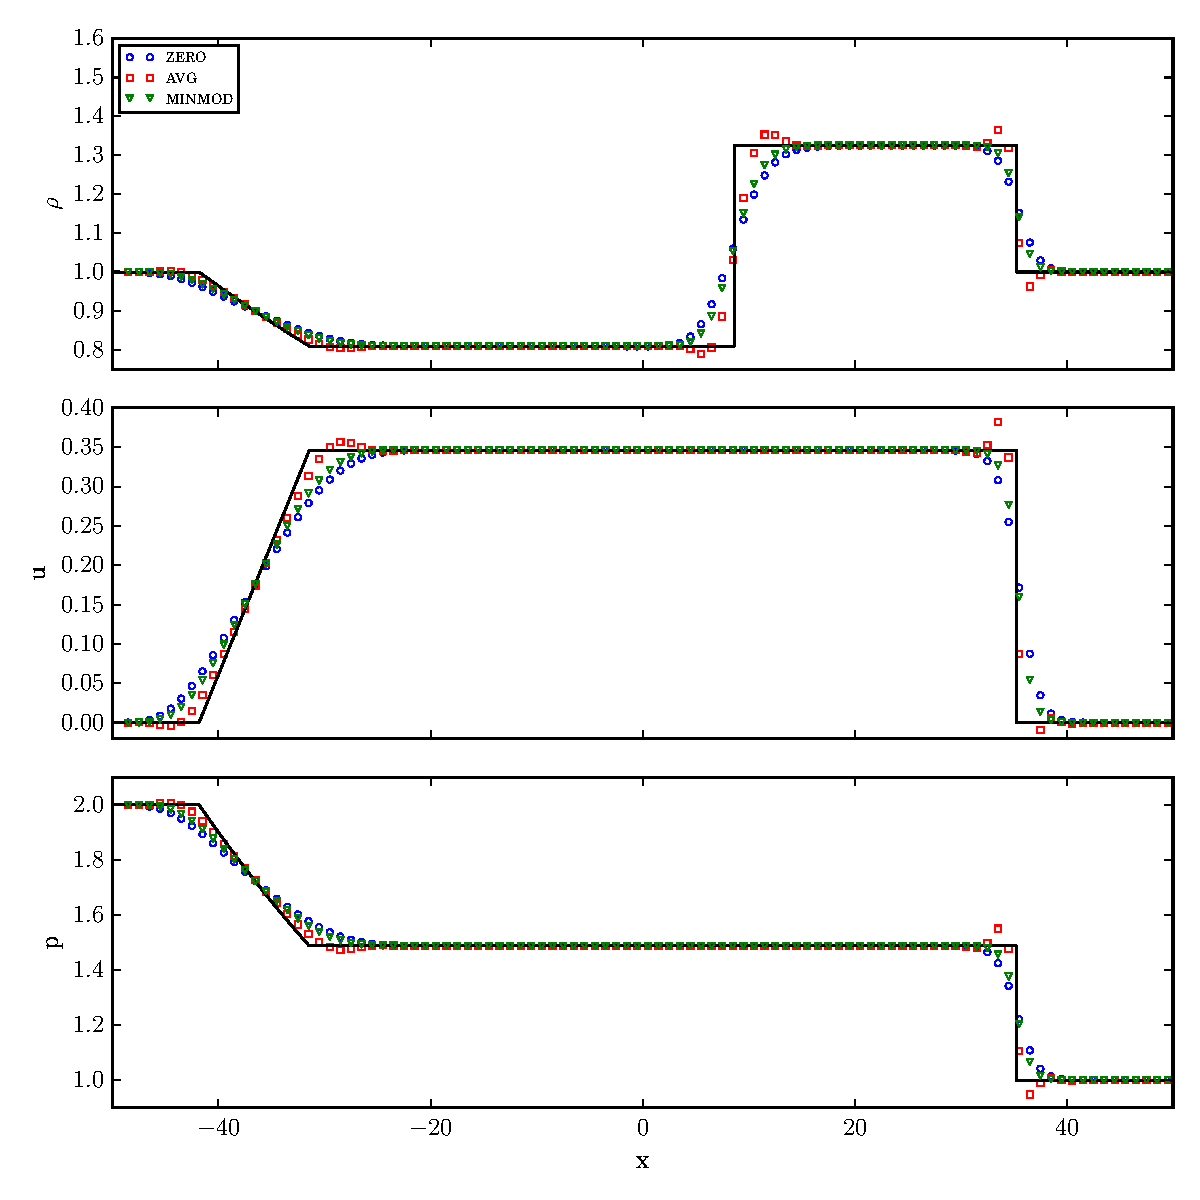
\includegraphics[width = \textwidth]{figures/task11.pdf}
    \caption{Effect of a slope limiter on the shock-tube problem.}
    \label{fig:task11}
\end{figure}

\subsection{Study of different limiters}
The MINDMOD, SUPERBEE and non-smooth Van-leer (VANLEERNS) slope limiters are compared in Fig. \ref{fig:task12}.
In the case of the one-dimensional Euler equations, there is little difference between the limiters.
Since the exact solution is comprised of discontinuous transitions, the most compressive limiter SUPERBEE performs the best with an $L_2$ error norm of 0.03793 on the density distribution.
VANLEERNS and MINMOD have $L_2$ error norms of 0.03866 and 0.03972 respectively.

\begin{figure}[htb]%
    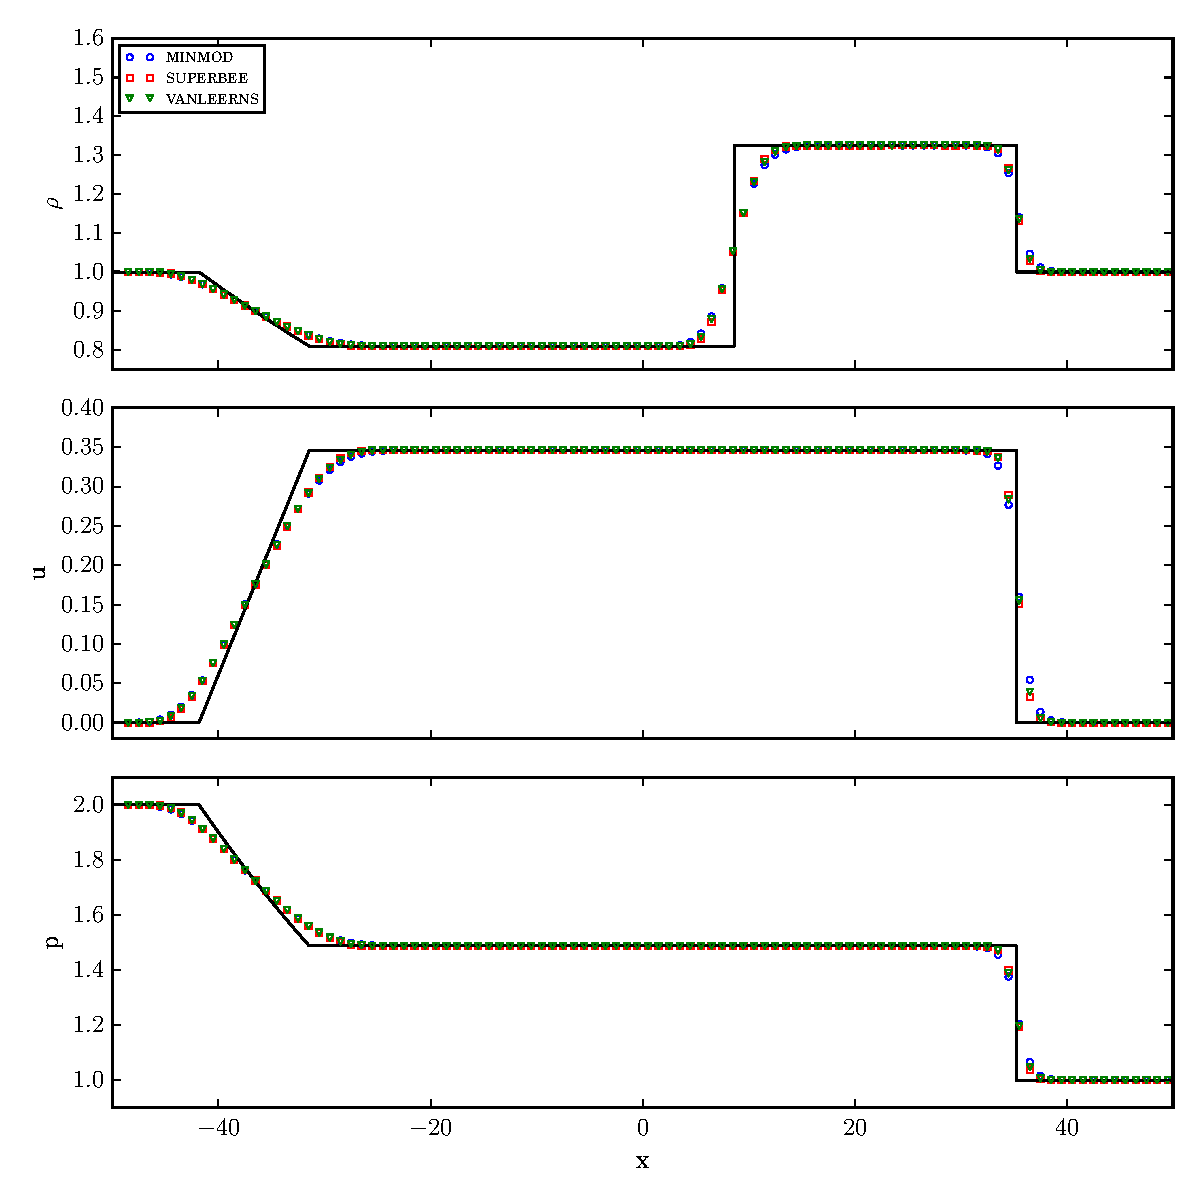
\includegraphics[width = \textwidth]{figures/task12.pdf}
    \caption{Comparison of slope limiters on the shock-tube problem.}
    \label{fig:task12}
\end{figure}

\section{Blast wave interaction with an wall}

The computational domain is defined from $x = 0$ to $x=1.5$ and solid wall boundary conditions are applied at the extremities through the use of halo cells.
Unless otherwise specified, 150 cells are used to evaluation the numerical solution and a CFL of 0.5 is used.
The SUPERBEE limiter is used for this numerical experiment.

Fig. \ref{fig:bwall}-\ref{fig:awall} show the numerical results before, during and after the wall interaction.
Before the wall interaction, the highly-pressurized area propagates through the rest of the domain, forming a right-facing shock.
As the gas expands, the density and pressure drop, while the gas moves to the right.

When the shock reaches the wall, a highly compressive region forms near the wall, and bounces back and forms a left-facing shock.
The shock interaction with the non-quiescent gas forms leads to an interesting behavior of the fluid density.
As the gas propagates back to the left, the pressurized region near the wall expands and decreases in pressure and density over time.

\begin{figure}[htb]%
    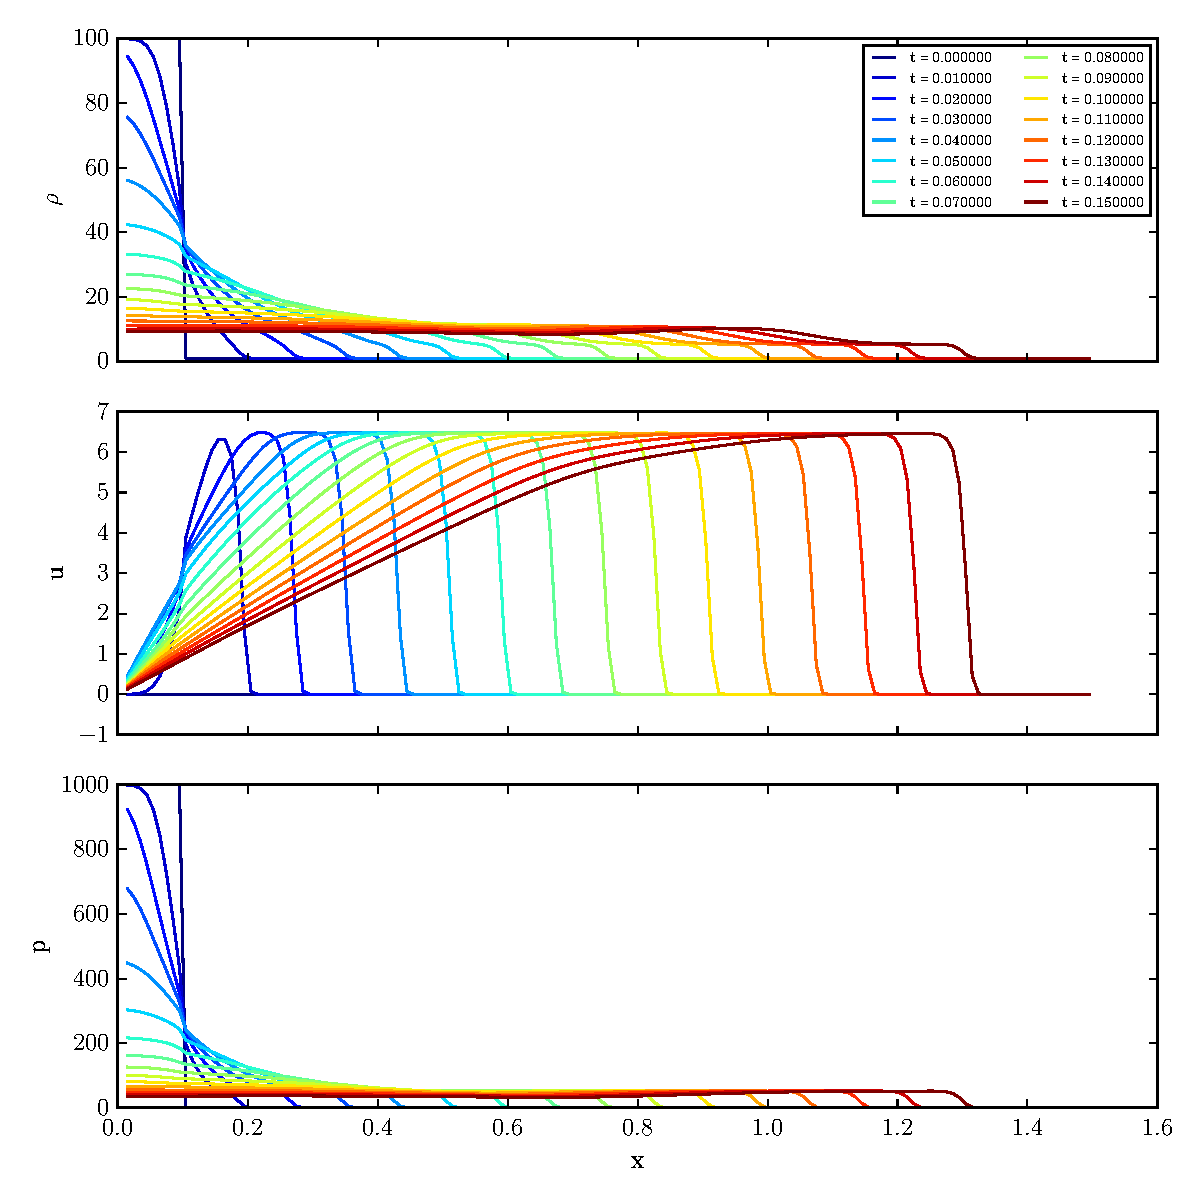
\includegraphics[width = \textwidth]{figures/beforewall.pdf}
    \caption{Before wall interaction}
    \label{fig:bwall}
\end{figure}

\begin{figure}[htb]%
    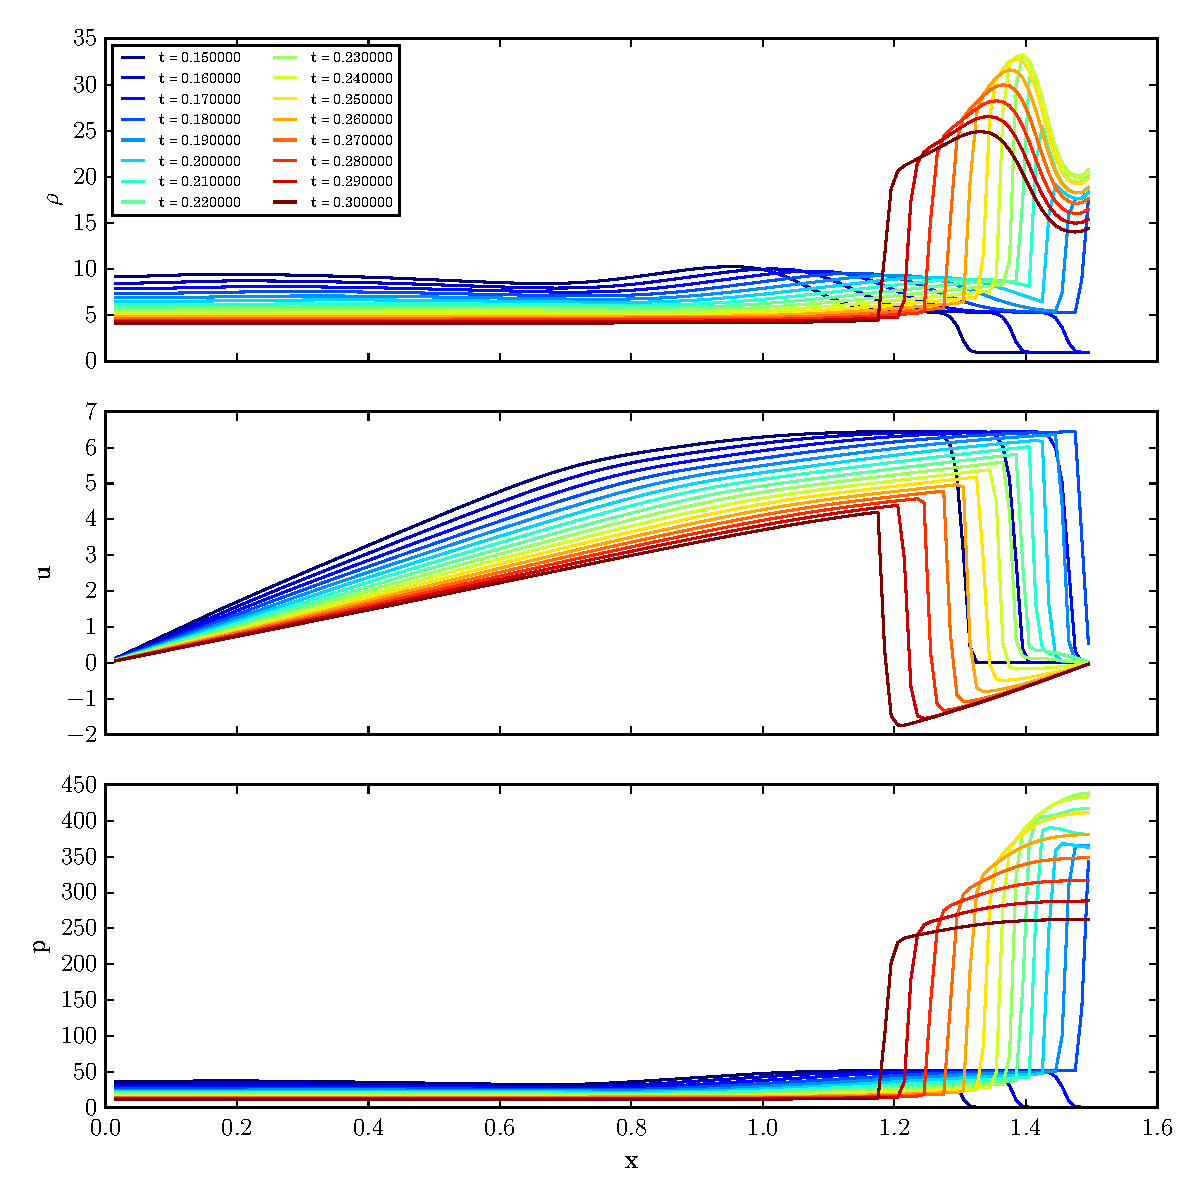
\includegraphics[width = \textwidth]{figures/duringwall.pdf}
    \caption{During wall interaction}
    \label{fig:dwall}
\end{figure}
\begin{figure}[htb]%
    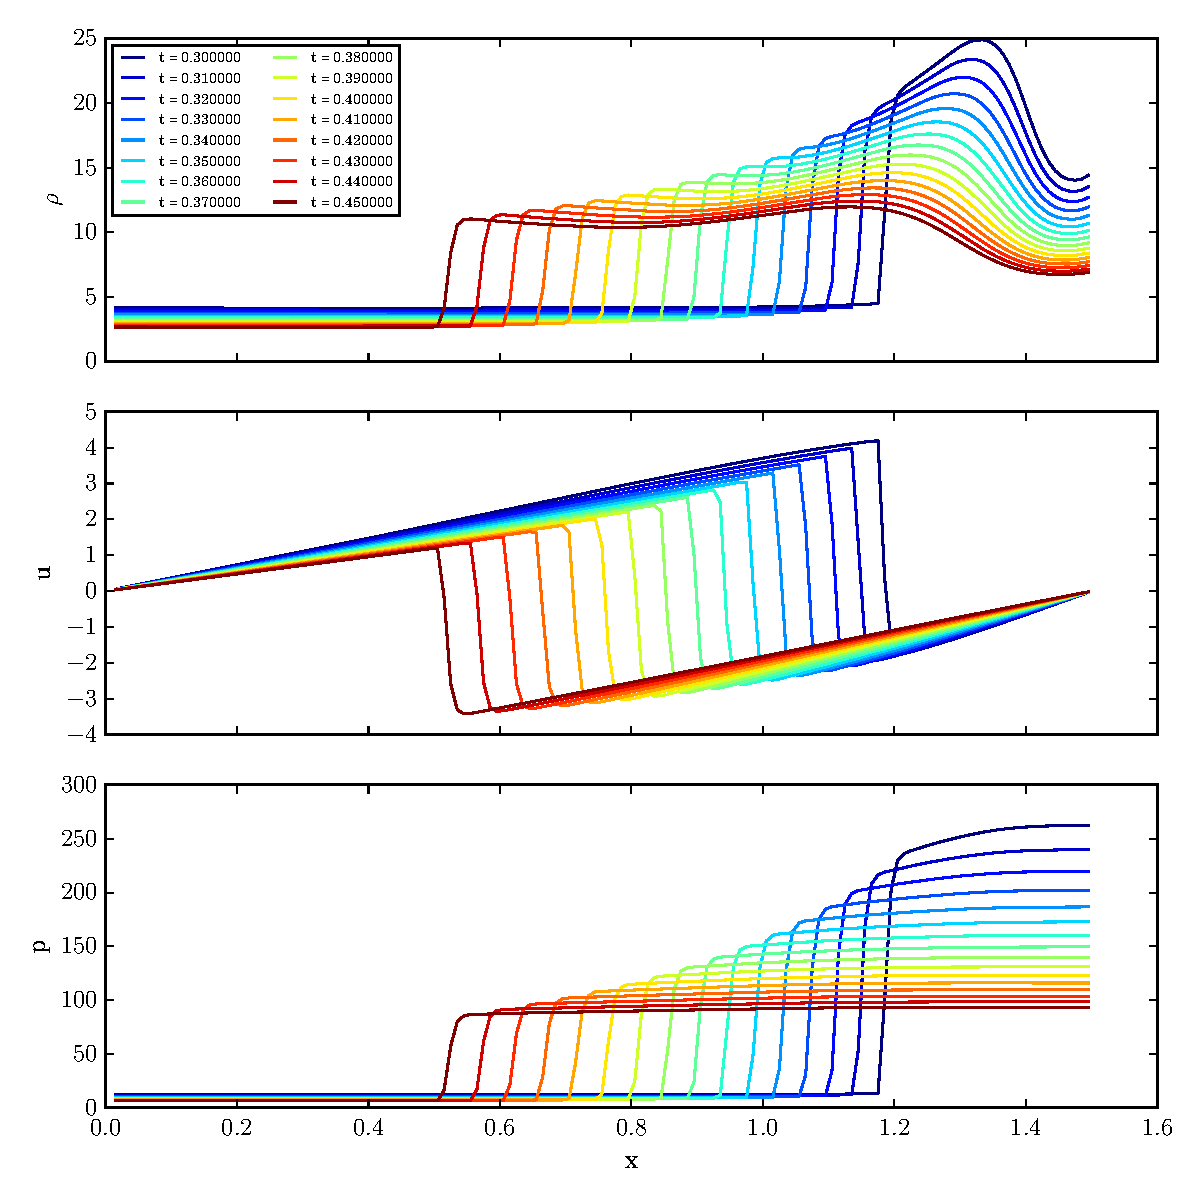
\includegraphics[width = \textwidth]{figures/afterwall.pdf}
    \caption{After wall interaction}
    \label{fig:awall}
\end{figure}

Let us consider $x = 1.3$ as a region of interest. Fig. \ref{fig:ptime} shows the pressure history for multiple grid sizes.
Around $t = 0.15$, the right-facing shock from the explosion makes the pressure rise at this location.
Pressure then diminishes as the gas keeps on expanding.
A second spike in pressure occurs when the left-facing shock comes back from the wall and results in the peak pressure at this location.
Fig. \ref{fig:peak} shows that as the mesh is refined, a maximum peak of approximately $p=326$ is attained.

\begin{figure}[htb]%
    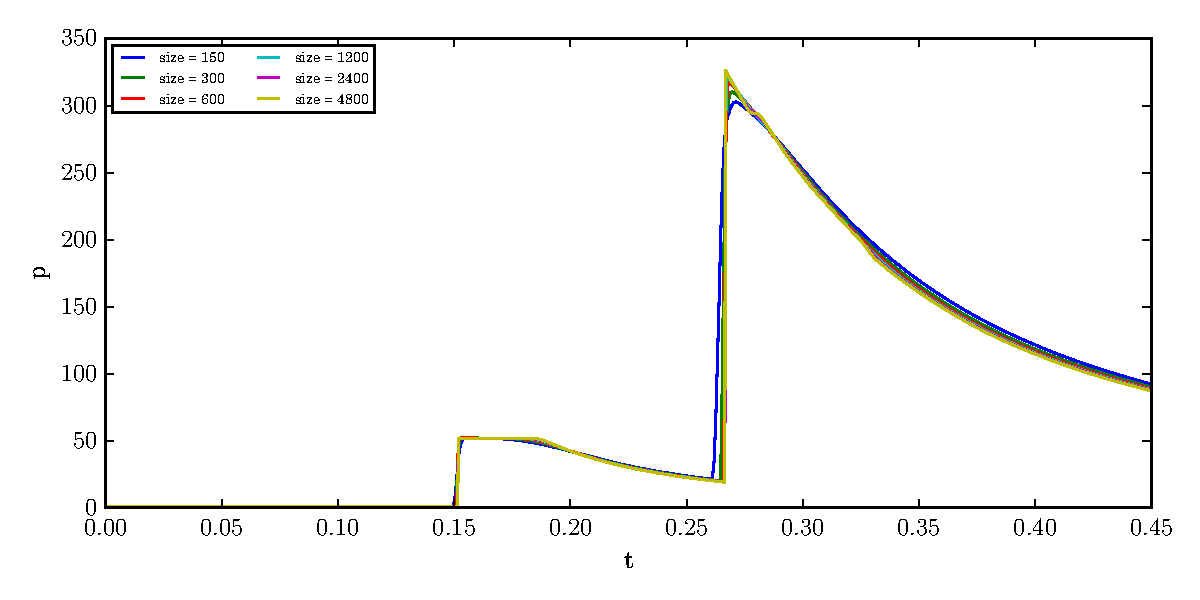
\includegraphics[width = \textwidth]{figures/pressuretime.pdf}
    \caption{Pressure history at $x = 1.3$}
    \label{fig:ptime}
\end{figure}
\begin{figure}[htb]%
    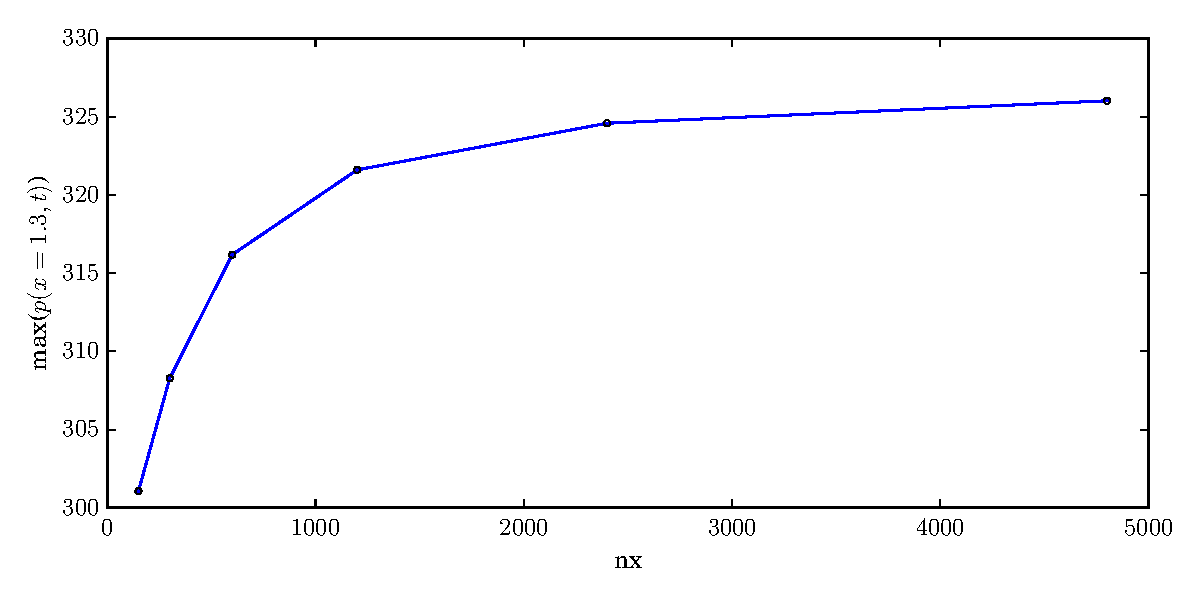
\includegraphics[width = \textwidth]{figures/pressurepeak.pdf}
    \caption{Peak pressure with grid refinement at $x = 1.3$}
    \label{fig:peak}
\end{figure}


\section*{Results and Code}

Code has been written in FORTRAN is available on my Github. The files have also been zipped with the report.

\url{https://github.com/dougshidong/mech516/tree/master/project3}


\end{document}
